% !TEX program = pdflatex
\RequirePackage[l2tabu, orthodox]{nag}
\documentclass{article}

% FONTS
\usepackage[T1]{fontenc}

% Replace default Latin Modern typewriter with its proportional counterpart
% http://www.tug.dk/FontCatalogue/lmoderntypewriterprop/
\renewcommand*\ttdefault{lmvtt}


%%% OPTION 1 - Fourier Math + New Century Schoolbook + ParaType Sans

% % Import Fourier Math (this imposes its own New Century Schoolbook type)
% % http://www.ctan.org/tex-archive/fonts/fouriernc/
% \usepackage{fouriernc}
% \usepackage{amsmath}
% % Replace with TeX Gyre Schola version of New Century Schoolbook (must scale!)
% % http://www.tug.dk/FontCatalogue/tgschola/
% \usepackage[scale=0.92]{tgschola}
% \usepackage[scaled=0.88]{PTSans}

%% OPTION 2 - MathDesign Math + Bitstream Charter + ParaType Sans

% Import MathDesign (this brings along Bitstream Charter)
% http://www.ctan.org/tex-archive/fonts/mathdesign/
\usepackage[bitstream-charter]{mathdesign}
\usepackage{amsmath}
\usepackage[scaled=0.92]{PTSans}


% %%% OPTION 3 - MTPRO 2 Math + Termes Times + ParaType Sans

% \usepackage{tgtermes}
% \usepackage{amsmath}
% \usepackage[subscriptcorrection,
%             amssymbols,
%             mtpbb,
%             mtpcal,
%             nofontinfo  % suppresses all warnings
%            ]{mtpro2}
% \usepackage{scalefnt,letltxmacro}
% \LetLtxMacro{\oldtextsc}{\textsc}
% \renewcommand{\textsc}[1]{\oldtextsc{\scalefont{1.10}#1}}
% \usepackage[scaled=0.92]{PTSans}

% GEOMETRY
\usepackage[
  paper  = letterpaper,
  left   = 1.65in,
  right  = 1.65in,
  top    = 1.0in,
  bottom = 1.0in,
  ]{geometry}

% COLOR
\usepackage[usenames,dvipsnames]{xcolor}
\definecolor{shadecolor}{gray}{0.9}

% SPACING and TEXT
\usepackage[final,expansion=alltext]{microtype}
\usepackage[english]{babel}
\usepackage[parfill]{parskip}
\usepackage{afterpage}
\usepackage{framed}

%redefine the leftbar environment to accept a width and coloring options
\renewenvironment{leftbar}[1][\hsize]
{%
  \def\FrameCommand
  {%
    {\color{Gray}\vrule width 3pt}%
    \hspace{10pt}%
    %\hspace{0pt}\fboxsep=\FrameSep\colorbox{black!10}%
  }%
  \MakeFramed{\hsize#1\advance\hsize-\width\FrameRestore}%
}%
{\endMakeFramed}

% define a paragraph header function
\DeclareRobustCommand{\parhead}[1]{\textbf{#1}~}

% EDITING
% line numbering in left margin
\usepackage{lineno}
\renewcommand\linenumberfont{\normalfont
                             \footnotesize
                             \sffamily
                             \color{SkyBlue}}
% ragged paragraphs in right margin
\usepackage{ragged2e}
\DeclareRobustCommand{\sidenote}[1]{\marginpar{
                                    \RaggedRight
                                    \textcolor{Plum}{\textsf{#1}}}}
% paragraph counter in right margin
\newcommand{\parnum}{\bfseries\P\arabic{parcount}}
\newcounter{parcount}
\newcommand\p{%
    \stepcounter{parcount}%
    \leavevmode\marginpar[\hfill\parnum]{\parnum}%
}
% paragraph helper
\DeclareRobustCommand{\PP}{\textcolor{Plum}{\P} }

% COUNTERS
\renewcommand{\labelenumi}{\color{black!67}{\arabic{enumi}.}}
\renewcommand{\labelenumii}{{\color{black!67}(\alph{enumii})}}
\renewcommand{\labelitemi}{{\color{black!67}\textbullet}}

% FIGURES
\usepackage{graphicx}
\usepackage[labelfont=bf]{caption}
\usepackage[format=hang]{subcaption}

% TABLES
\usepackage{booktabs}

% ALGORITHMS
\usepackage[algoruled]{algorithm2e}
\usepackage{listings}
\usepackage{fancyvrb}
\fvset{fontsize=\normalsize}

% BIBLIOGRAPHY
\usepackage{natbib}

% HYPERREF
\usepackage[colorlinks,linktoc=all]{hyperref}
\usepackage[all]{hypcap}
\hypersetup{citecolor=BurntOrange}
\hypersetup{linkcolor=MidnightBlue}
\hypersetup{urlcolor=MidnightBlue}

% CLEVEREF must come after HYPERREF
\usepackage[nameinlink]{cleveref}

% ACRONYMS
\usepackage[acronym,smallcaps,nowarn]{glossaries}
% \makeglossaries

% COLOR DEFINITIONS
\newcommand{\red}[1]{\textcolor{BrickRed}{#1}}
\newcommand{\orange}[1]{\textcolor{BurntOrange}{#1}}
\newcommand{\green}[1]{\textcolor{OliveGreen}{#1}}
\newcommand{\blue}[1]{\textcolor{MidnightBlue}{#1}}
\newcommand{\gray}[1]{\textcolor{black!60}{#1}}

% LISTINGS DEFINTIONS
\lstdefinestyle{mystyle}{
    commentstyle=\color{OliveGreen},
    keywordstyle=\color{BurntOrange},
    numberstyle=\tiny\color{black!60},
    stringstyle=\color{MidnightBlue},
    basicstyle=\ttfamily,
    breakatwhitespace=false,
    breaklines=true,
    captionpos=b,
    keepspaces=true,
    numbers=left,
    numbersep=5pt,
    showspaces=false,
    showstringspaces=false,
    showtabs=false,
    tabsize=2
}
\lstset{style=mystyle}


\DeclareRobustCommand{\mb}[1]{\ensuremath{\boldsymbol{\mathbf{#1}}}}

\DeclareMathOperator*{\argmax}{arg\,max}
\DeclareMathOperator*{\argmin}{arg\,min}

\DeclareRobustCommand{\KL}[2]{\ensuremath{\textrm{KL}\left(#1\;\|\;#2\right)}}

\newcommand{\mbx}{\mathbold{x}}
\newcommand{\mbX}{\mbf{X}}

\newcommand{\mbz}{\mathbold{z}}

\newcommand{\mbI}{\mbf{I}}

\newcommand{\mbZ}{\mbf{Z}}
\newcommand{\mbL}{\mbf{L}}

\newcommand{\mbtheta}{\mathbold{\theta}}
\newcommand{\mbTheta}{\mathbold{\Theta}}
\newcommand{\mbomega}{\mathbold{\omega}}
\newcommand{\mbOmega}{\mathbold{\Omega}}
\newcommand{\mbsigma}{\mathbold{\sigma}}
\newcommand{\mbSigma}{\mathbold{\Sigma}}

\newcommand{\mblambda}{\mathbold{\lambda}}
\newcommand{\mbgamma}{\mathbold{\gamma}}
\newcommand{\mbzeta}{\mathbold{\zeta}}
\newcommand{\mbeta}{\mathbold{\eta}}
\newcommand{\mbbeta}{\mathbold{\beta}}
\newcommand{\mbphi}{\mathbold{\phi}}
\newcommand{\mbmu}{\mathbold{\mu}}
\newcommand{\mbrho}{\mathbold{\rho}}

\newcommand\dif{\mathop{}\!\mathrm{d}}
\newcommand{\diag}{\textrm{diag}}
\newcommand{\supp}{\textrm{supp}}

\newcommand{\E}{\mathbb{E}}
\newcommand{\Var}{\mathbb{V}\textrm{ar}}

\newcommand{\bbN}{\mathbb{N}}
\newcommand{\bbZ}{\mathbb{Z}}
\newcommand{\bbR}{\mathbb{R}}
\newcommand{\bbS}{\mathbb{S}}

\newcommand{\cL}{\mathcal{L}}

\newcommand{\cN}{\mathcal{N}}
\newcommand{\Gam}{\textrm{Gam}}
\newcommand{\InvGam}{\textrm{InvGam}}

\newacronym{KL}{kl}{Kullback-Leibler}
\newacronym{ELBO}{elbo}{\emph{evidence lower bound}}
\newacronym{POPELBO}{pop-elbo}{\emph{population evidence lower bound}}

\newacronym{SVI}{svi}{stochastic variational inference}
\newacronym{BUMPVI}{bump-vi}{bumping variational inference}

\newacronym{GMM}{gmm}{Gaussian mixture model}
\newacronym{LDA}{lda}{latent Dirichlet allocation}

\newacronym{SUTVA}{sutva}{stable unit treatment value assumption}


% \linenumbers
\DeclareMathOperator*{\Categorical}{Categorical}


\title{Generative Models for scRNA}
\author{Jackson Loper}

\usepackage{amsthm}
\newtheorem{thm}{Theorem}
\newtheorem{conj}{Conjecture}

\begin{document}
\maketitle

\begin{description}
  \item[Status] Succesfully trained the new ``iterative model,'' evaluated it to some extent
  \item[Todo] Compare clusters against Allen, consider linear model, do more layers
\end{description}

\section{Overview}

The Allen Institute has developed a method for clustering, one that has apparently allowed them to distinguish 116 unique cell types using single cell RNA data.  The method follows the following recursive procedure:

\begin{algorithm}[H]
 \KwData{RNA expression for a collection of cells}
 \vspace{.1in}
  Run PCA on the data (e.g. take first 16 components)\;
  Run T-SNE on the resulting low-d representation\;
  Circle things that look like clusters\;
  \If{there is more than one cluster}{\For{each cluster $c$}{run itclust on the cells inside $c$\;}}
 \caption{itclust}
\end{algorithm}

This method is nice because the important low-dimensional representations \emph{within} a cluster may be quite different from the ones that help you distinguish \emph{between} two subclusters within that cluster.  This is what allows them to achieve the level of granularity that they have. 

Unfortunately, it is a bit difficult to grasp the uncertainty involved in the process.  There is certainly noise in the data, and different practitioners of this basic procedure may have different understandings of what this noise is.  The result is that when Bosilijka Tasic (one of the lead experimentalists at Allen) gives two data scientists the same data, they each come back with different answers.  And they have no way to compare or evaluate these two different answers.  One essential question is ``what level of granularity does the signal-to-noise ratio support?''  The algorithm above, as stated, runs iteratively until subclusters cannot be distinguished via T-SNE.  But this is obviously a very subjective matter.  What to do?

We propose to help clarify some of these issues by building a fully generative model of gene expression, one that rigorously measures some kinds of uncertainty in every step of the process.  To be most useful to the Allen Institute, however, we also want this generative model to fit into the scientific paradigm under which they are operating.  In particular, the treatment of clusters should be hierarchical in nature, and it is desirable that the model have latent representations that roughly correspond to the low-dimensional representations found in the Allen algorithm.  

\section{Model}

\begin{figure}
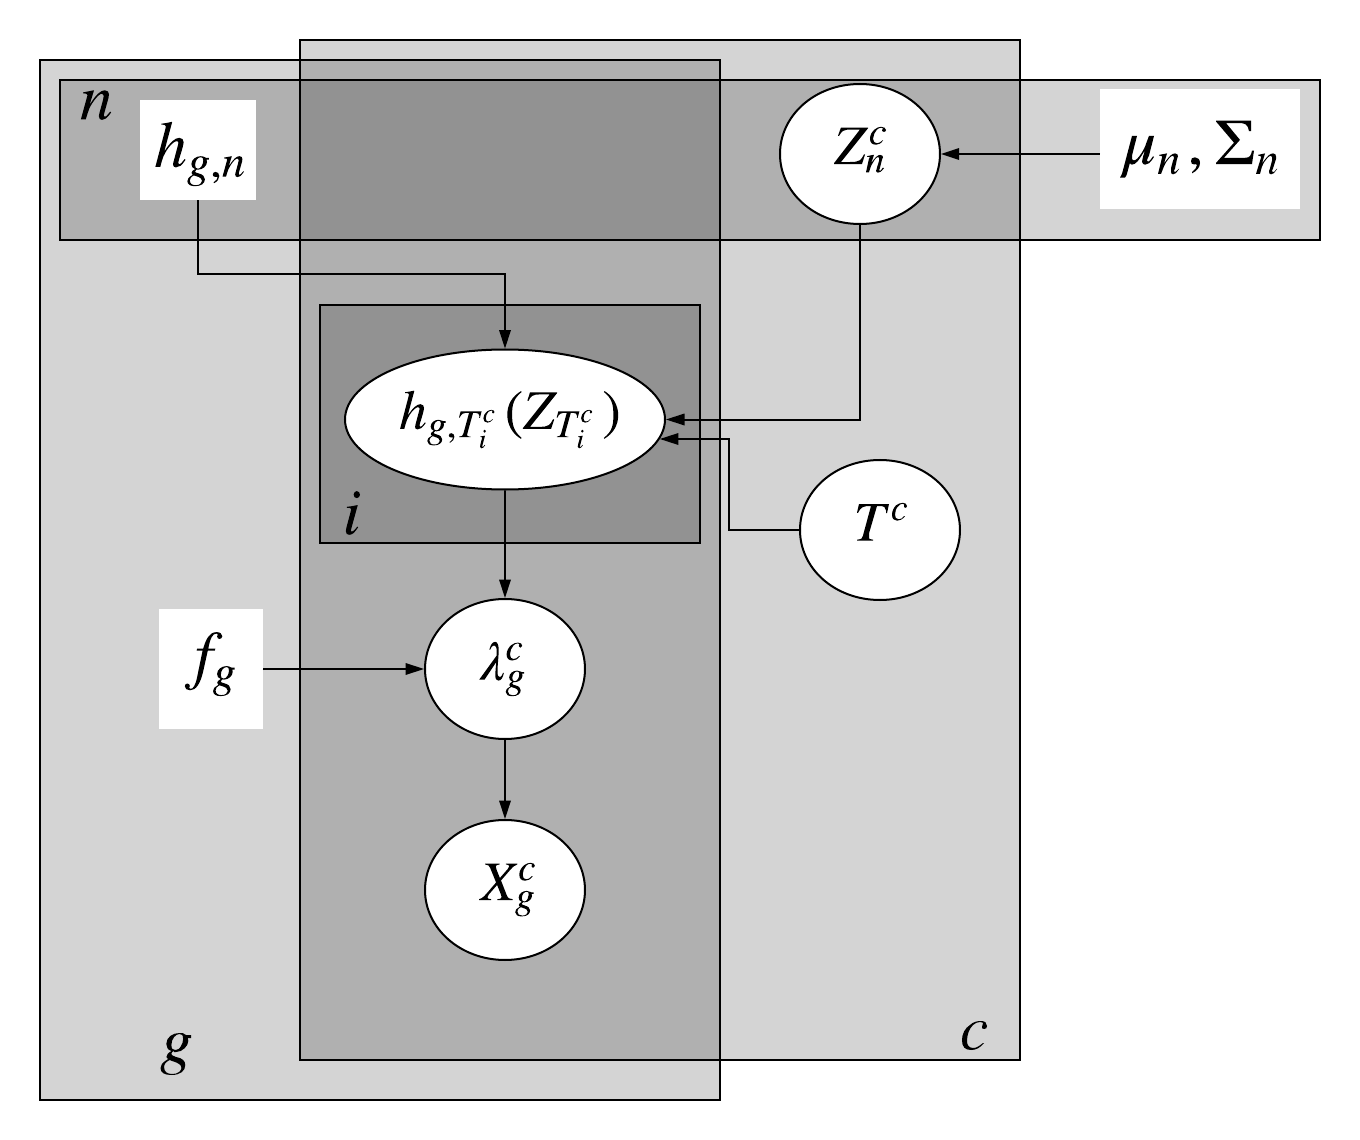
\includegraphics[width=0.8\textwidth]{pics/plate}
\caption{Plate diagram for the model\label{fig:plate}.  $i$ indexes layers of the hierarchy of cell types, $n$ indexes nodes in the hierarchy of cell types,  $c$ indexes cells, and $g$ indexes genes.}
\end{figure}

Towards this end, we propose the following generative model for gene expression of a single cell.  We will denote the expression of gene $g$ in cell $c$ by $X_g^c$.  Let $H$ denote a tree of cell types.   

\begin{enumerate}
\item $T^c \sim \Categorical(\pi)$, one of the leaves of $H$.  Let $t_0,t_1(T^c),t_2(T^c),\cdots ,t_\ell^c(T^c)$, indicate the nodes in the unique path in $H$ which leads from the root to the leaf $T$.  Here $t_0$ is the root of the tree, $\ell^c$ is the depth of the leaf $T^c$, and $t^c_\ell(T^c)=T^c$.   To consolidate notation, we take $T^c_i \triangleq t_i(T^c)$.
\item For each $i<\ell$ let $Z^c_{T^c_i} \sim \cN(\mu_{T^c_{i+1}},\Sigma_{T^c_{i+1}})$, and take $Z^c_{T^c_\ell} \sim \cN(0,I)$
\item For each gene $g$, let $\lambda^c_g \in \mathbb R^{p}$ denote a set of parameters.  These will be a deterministic function of the $Z$s:
\[
\lambda^c_g = f_g \left(\sum_{i=0}^{\ell} h_{g,T^c_i}(Z^c_{T^c_i})\right)
\]
\item Conditioned on $Z^c$ we will have $X^c_g \sim p(x_g ; \lambda^c_g)$. 
\end{enumerate}

This can be a bit confusing to take in.  The plate diagram in Figure \ref{fig:plate} may help.  We can also try to unpack some of this in words:

\begin{itemize}
\item The latent representation $Z^c_i$ corresponds to features of that cell which are specific to all the cells which are descendents of $T^c_i$.
\item The the cell's subcluster $T^c_{i+1}$ effects the distribution of its latent features at the $i$th level, $Z^c_i$.  That is, the latent distribution on the $i$th latent representation is governed by what subcluster it is part of within $T^c_i$.
\item The distribution of the final latent representation, $Z^c_T$, is simply a standard normal.
\item The functions $h_{g,T^c_i}$ indicates how these cell-type-specific features alter the distribution on the gene expressions for cells in that branch of the tree.  
\end{itemize}

For inference, we use amortized variational inference.  In particular, we take the variational family that $T$ and all the $Z_{T_i}$ are independent, $T$ is some categorical, and $Z$s are isotropic gaussians.  We build a neural network to estimate the variational parameters from gene expressions.  Note that this network must estimate the parameters for a gaussian at \emph{each node} in the tree $H$.

\section{Empirical results}

At the current moment, we have only actually implemented this model in the case the $H$ is a tree with depth 2 (i.e. one root node and some children).  We take the data model to be a zero-inflated negative binomial.  It looks fairly promising.  For a simple qualitative assessment, consider the following.

Scatterplot of the aggregate posterior distribution of $Z_{T_0}$, colored by posterior mean of the cluster assigment.  That is, each dot is a cell, its position is given by a posterior sample of $Z_{T_0}$, and its color has something to do with what cluster we expect it to be in.  

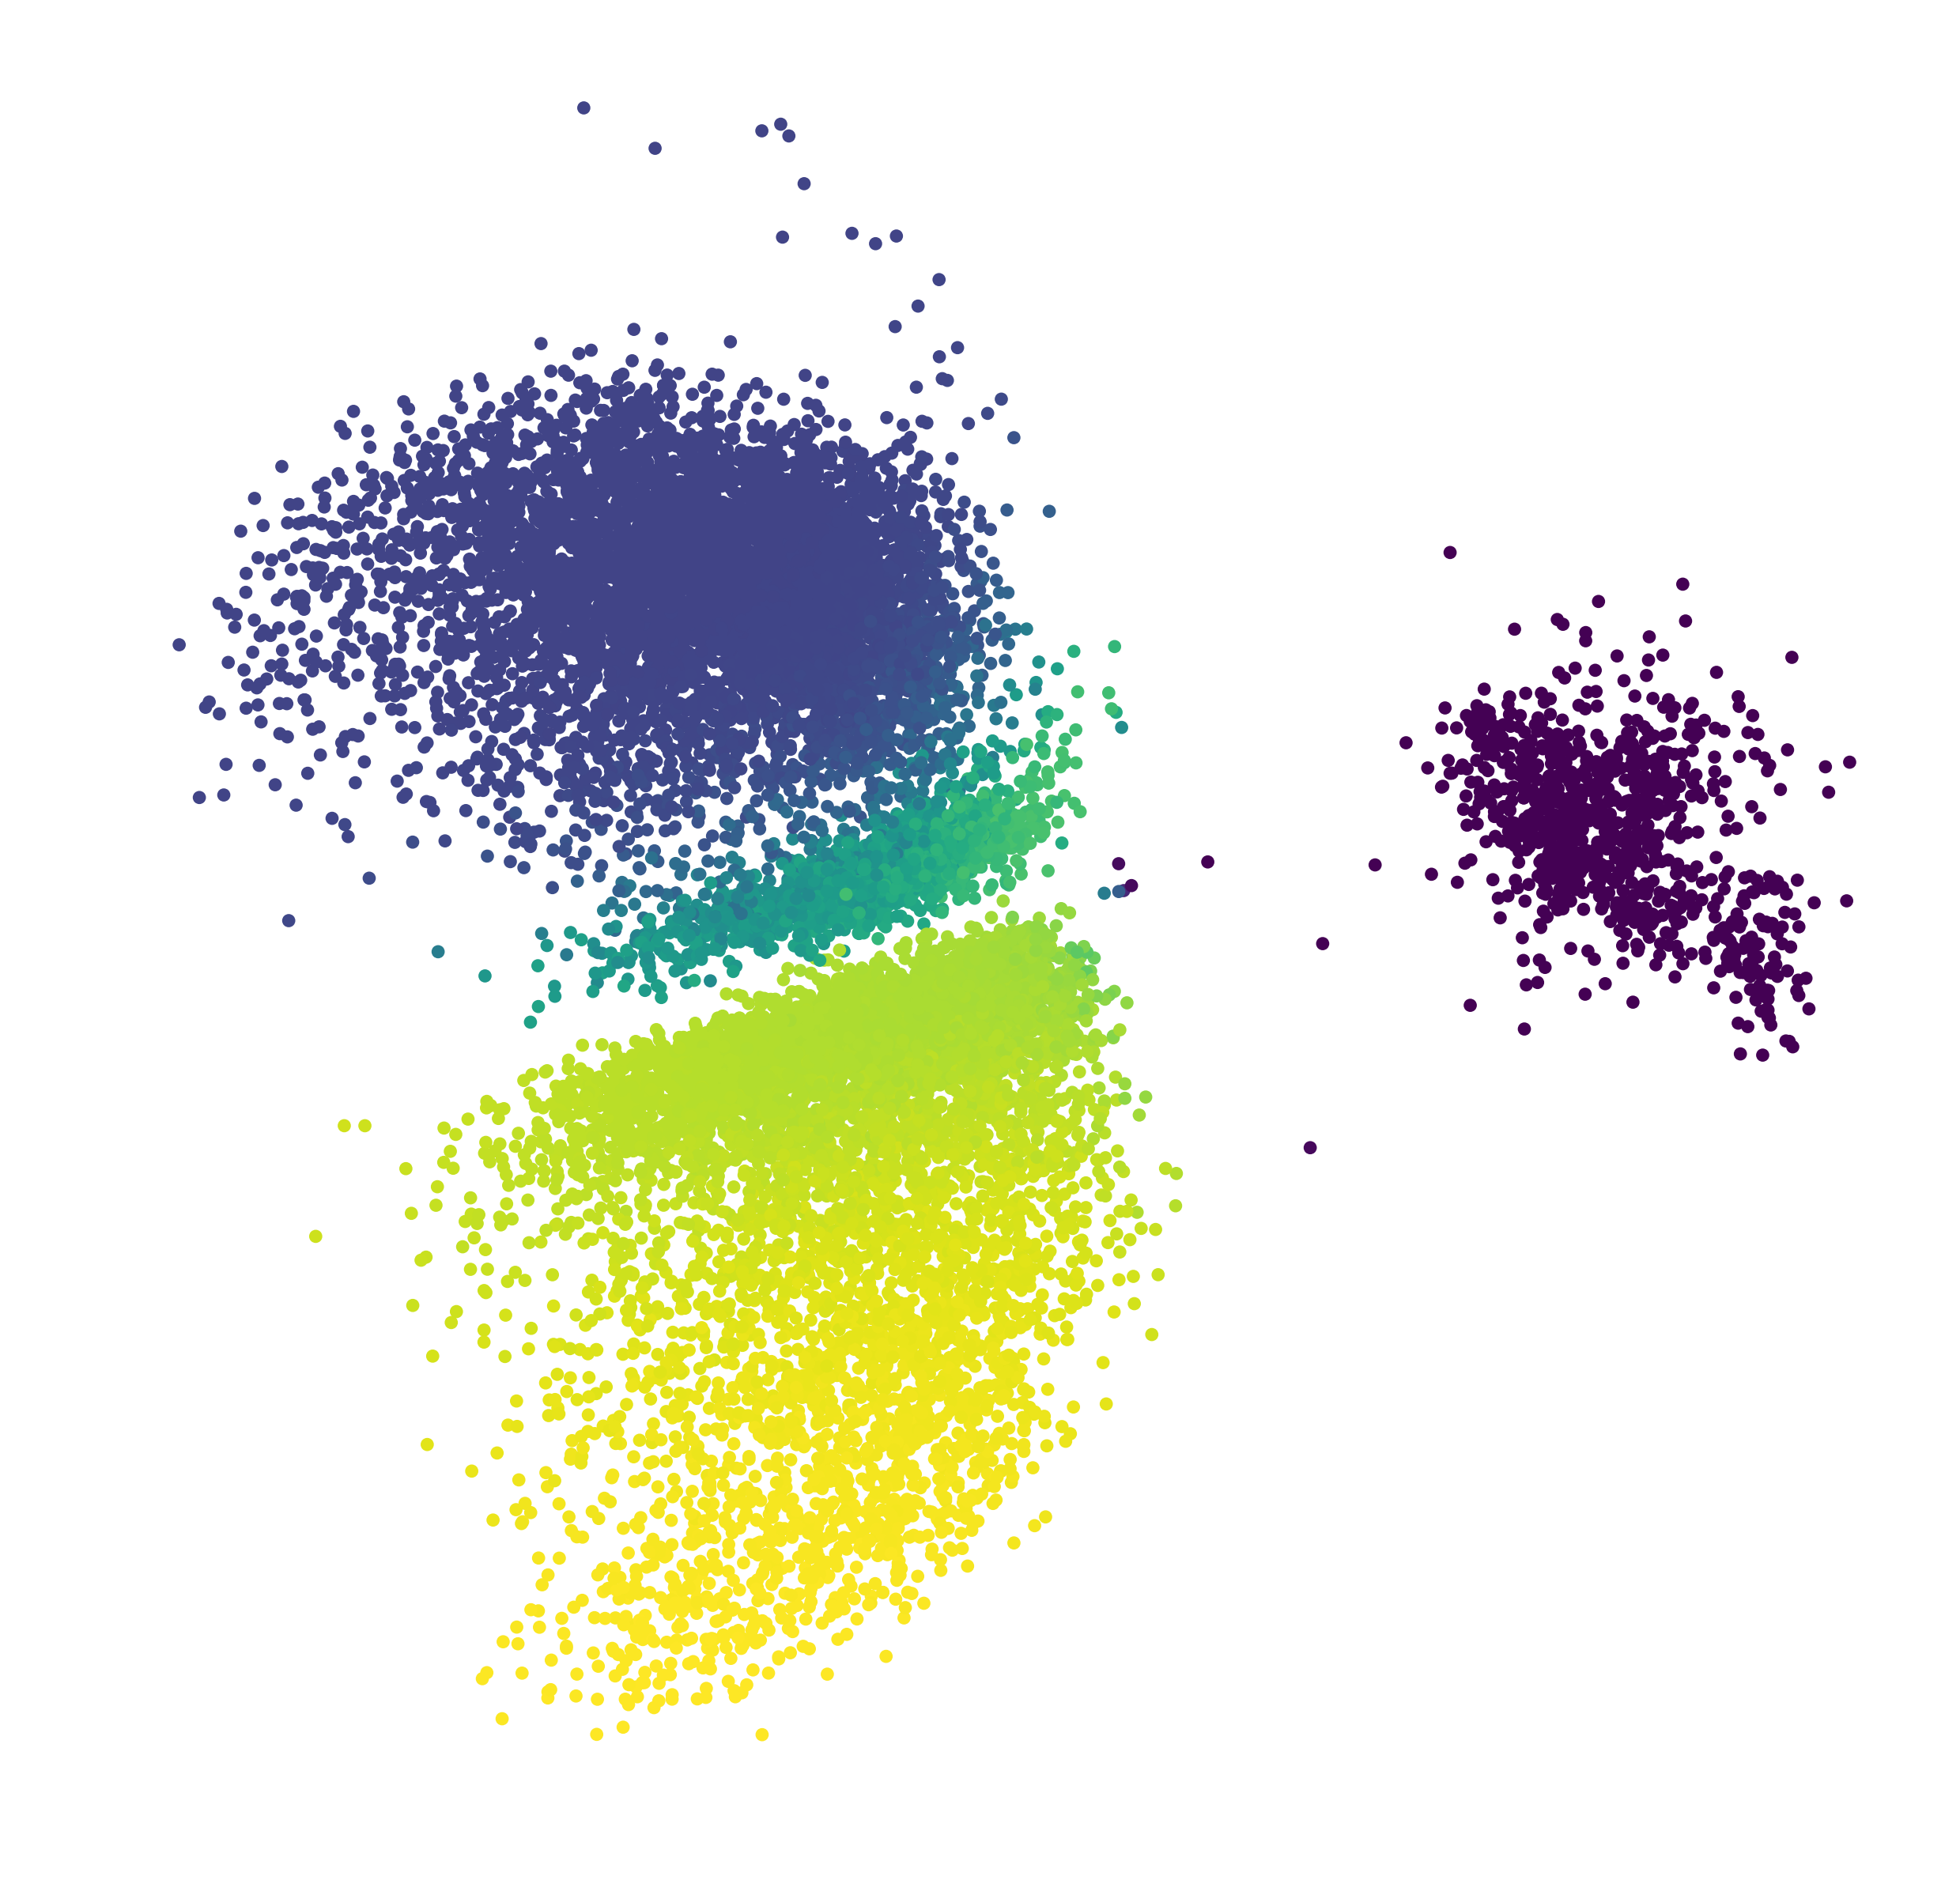
\includegraphics[width=0.4\textwidth]{pics/Z1}

Notice that there are only so many clusters that are really clearly distinct in this latent space.  However, let's focus on that cluster on the right-hand side.  What happens if we look at the $Z_{T_1}$ variables for those cells?  We get substantial subclustering apparent in the $Z_{T_1}$ space.  In the following picture, each dot is a cell from the cluster on the right-hand-side of the previous figure, and the position is given by a posterior sample of $Z_{T_1}$.

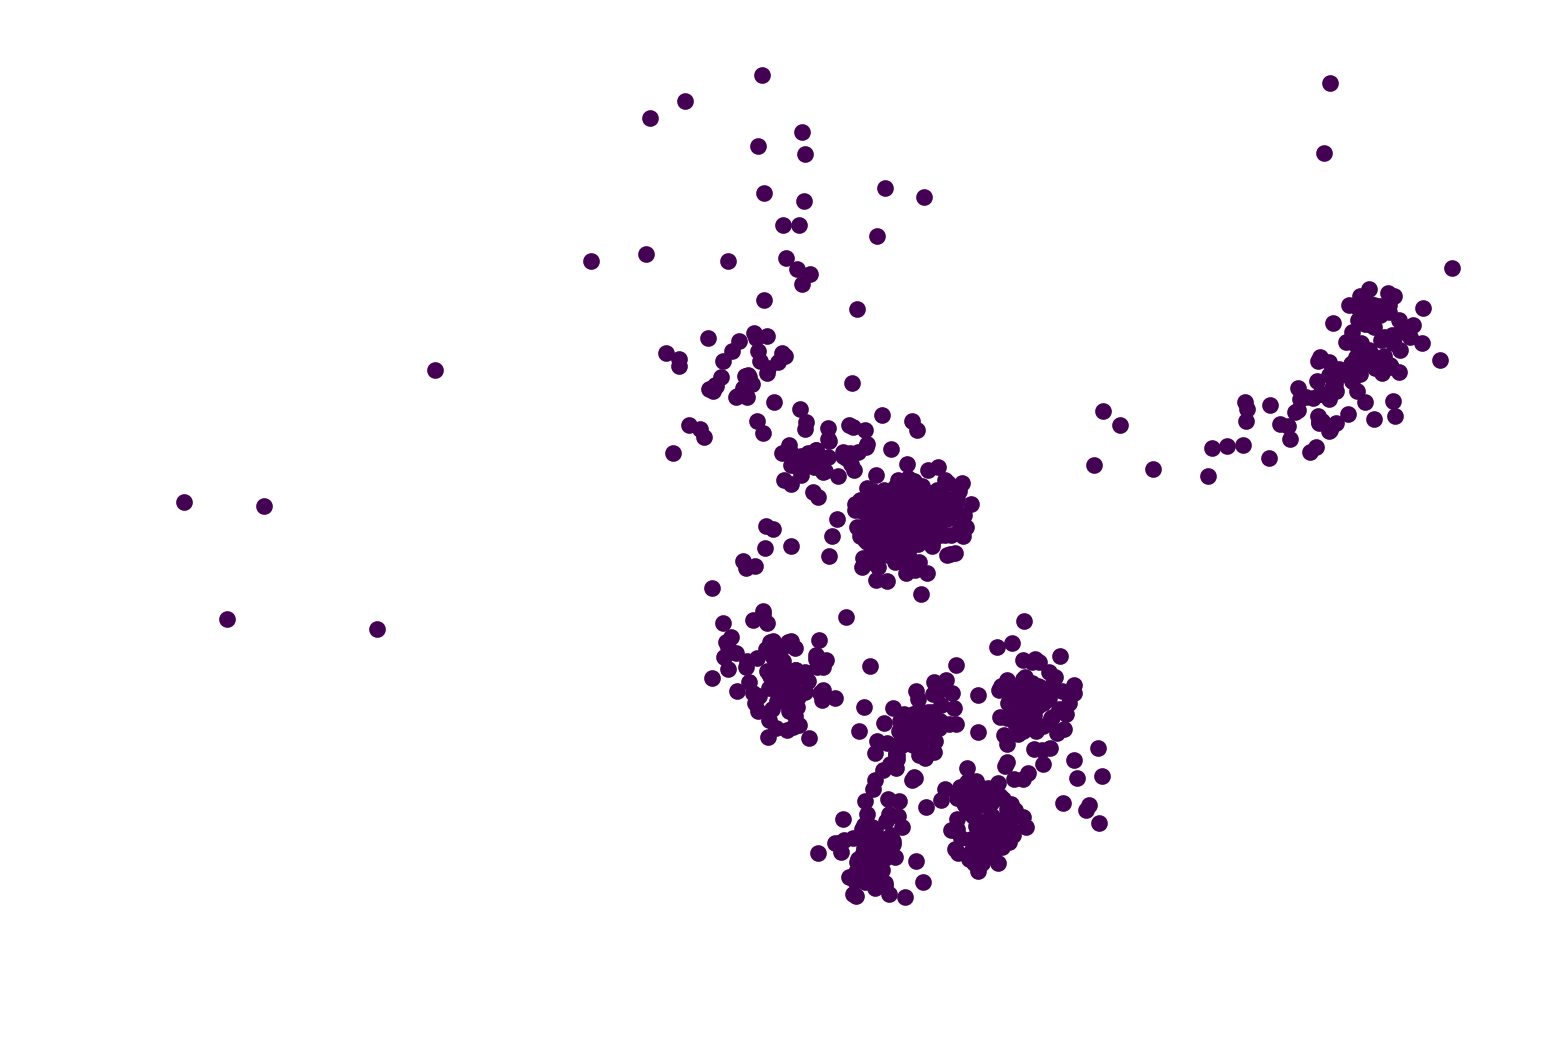
\includegraphics[width=0.4\textwidth]{pics/Z2}


\subsection{Held out log likelihood}

To quantitatively analyse our method, we used a held out log likelihood:

\begin{itemize}
\item Train the method on 75\% of the cells
\item For each of the remaining 25\% of the cells, select 75\% of the genes (``observed''):
  \begin{itemize}
  \item Compute the posterior mode of Z given the expression of those genes
  \item Compute the log probability of the observed genes given the posterior mode
  \item Compute the log probability of the unobserved genes given the posterior mode
  \end{itemize}
\item Average values over those 25\% of the cells
\end{itemize}

Here are the results for this ``Posterior mode predictive (PMP)'' approach:

\begin{tabular}{r|cc}
Method & PMP, observed & PMP, unobserved \\
Factor analysis $k=16$ & -4.2 & -4.2 \\
Factor analysis $k=64$ & -4.1 & -4.3 \\
HNBPF $k=2$ & -5.7 & -5.7 \\
HNBPF $k=16$ & -3.8 & -3.9 \\
HNBPF $k=64$ & -3.8 & -5.7 \\
ZINB-Vae $k=2$ & -3.6 & -3.6 \\
Smooth ZINB-Vae $k=2$ & -3.6 & -3.6 \\
Smooth Hierarchical ZINB $k=2+2$ & -3.5 & -3.5 \\
\hline
\end{tabular}

Here HNBPF is a negative-binomial-poisson-factorization approach, ZINB-Vae is based on a Michael Jordan paper, $k$ is the number of latent dimensions.  The results are certainly not mind-blowing, but its nice to see that we're at least not doing worse.  

To do posterior inference on held out likelihood, our approach is to first set all of the ``unobserved'' entries to the average value for the corresponding genes, and apply our inference network unchanged to get estimates for the variational parameters.  We then refine these estimates with gradient descent.  We note that if we use completely random guesses to initialize the gradient descent, we often converge to inferior local minima; this shows the benefit of the amortized inference.  

\subsection{Posterior predictive samples}

One limitation of the method as we have implemented it is that the posterior predictive distribution seems to be substantially underfitting.  To see what we mean, consider the following figure:

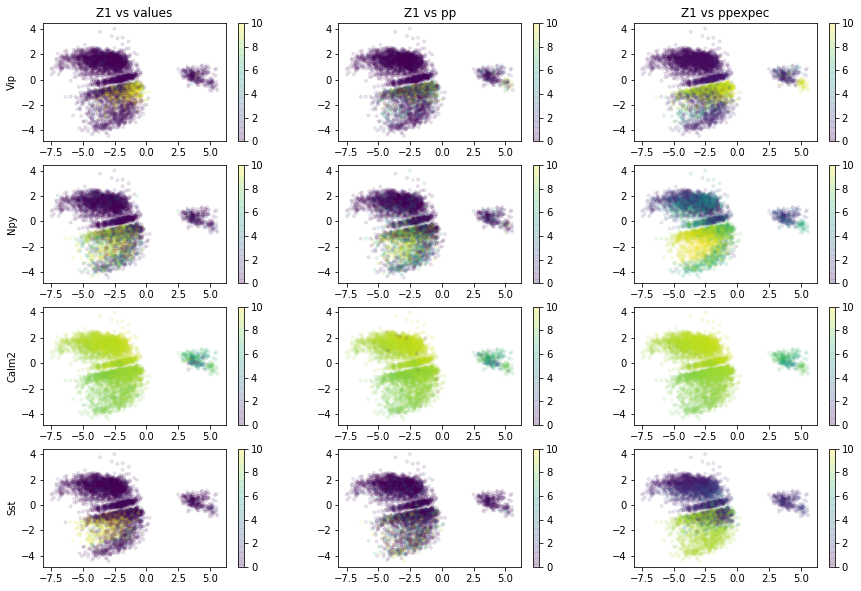
\includegraphics[width=0.8\textwidth]{pics/Z1gn}

Here we four rows and three columns of plots.  Each row corresponds to a different gene.  Each dot in each plot corresponds to a cell.  The position of the dot indicates the latent representation of the cell, as inferred by posterior inference.  The color indicates the amount of expression for the particular gene for that cell, measured three ways:

\begin{enumerate}
\item The first column shows the true expression of the appropriate gene for each cell (i.e the color of each dot is the gene expression for that cell)
\item The second column shows a posterior predictive sample of the gene expression for each cell
\item The third column shows the mean of such samples for each cell
\end{enumerate}

We see that the true expression doesn't match the posterior predictive expression for the Vip and Sst genes as well as we might like.  Something better is needed.  Possibly more layers.  Possibly more training.  Worth thinking about.

Another way to see that the model isn't quite right is to look at posterior predictive p values.  That is, for each entry of the matrix, we can compute the cumulative distribution function of that entry in light of the parameters predicted by the posterior mode.  Here we have done that for the first 1000 entries.  

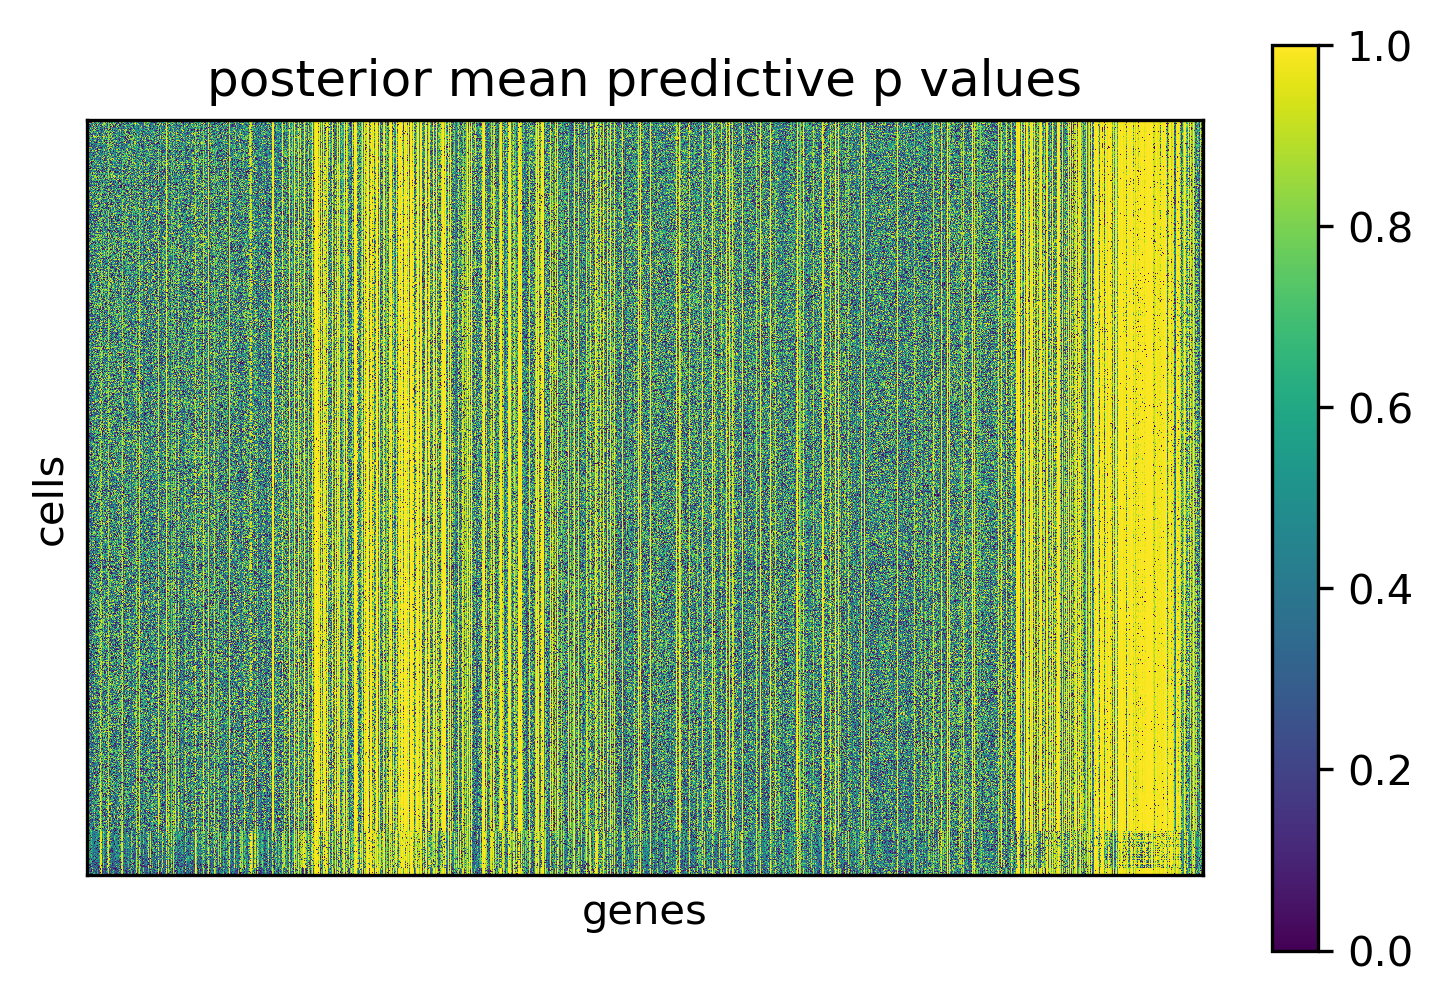
\includegraphics[width=0.8\textwidth]{pics/resids}

These results are actually fairly encouraging.  Mostly it looks basically like white noise.  However, we do see that for some genes the $p$ values are almost always near 1: these are genes which express essentially never, and so have a high chance of turning off, and so their $p$ value is nearly $1$ whenever they are off, which is virtually always.  

Anotehr way to dig deeper into the underfitting question is by looking at individual genes, and comparing the expected value for that gene under the model with the actual value.  There are clearly some systematic differences:

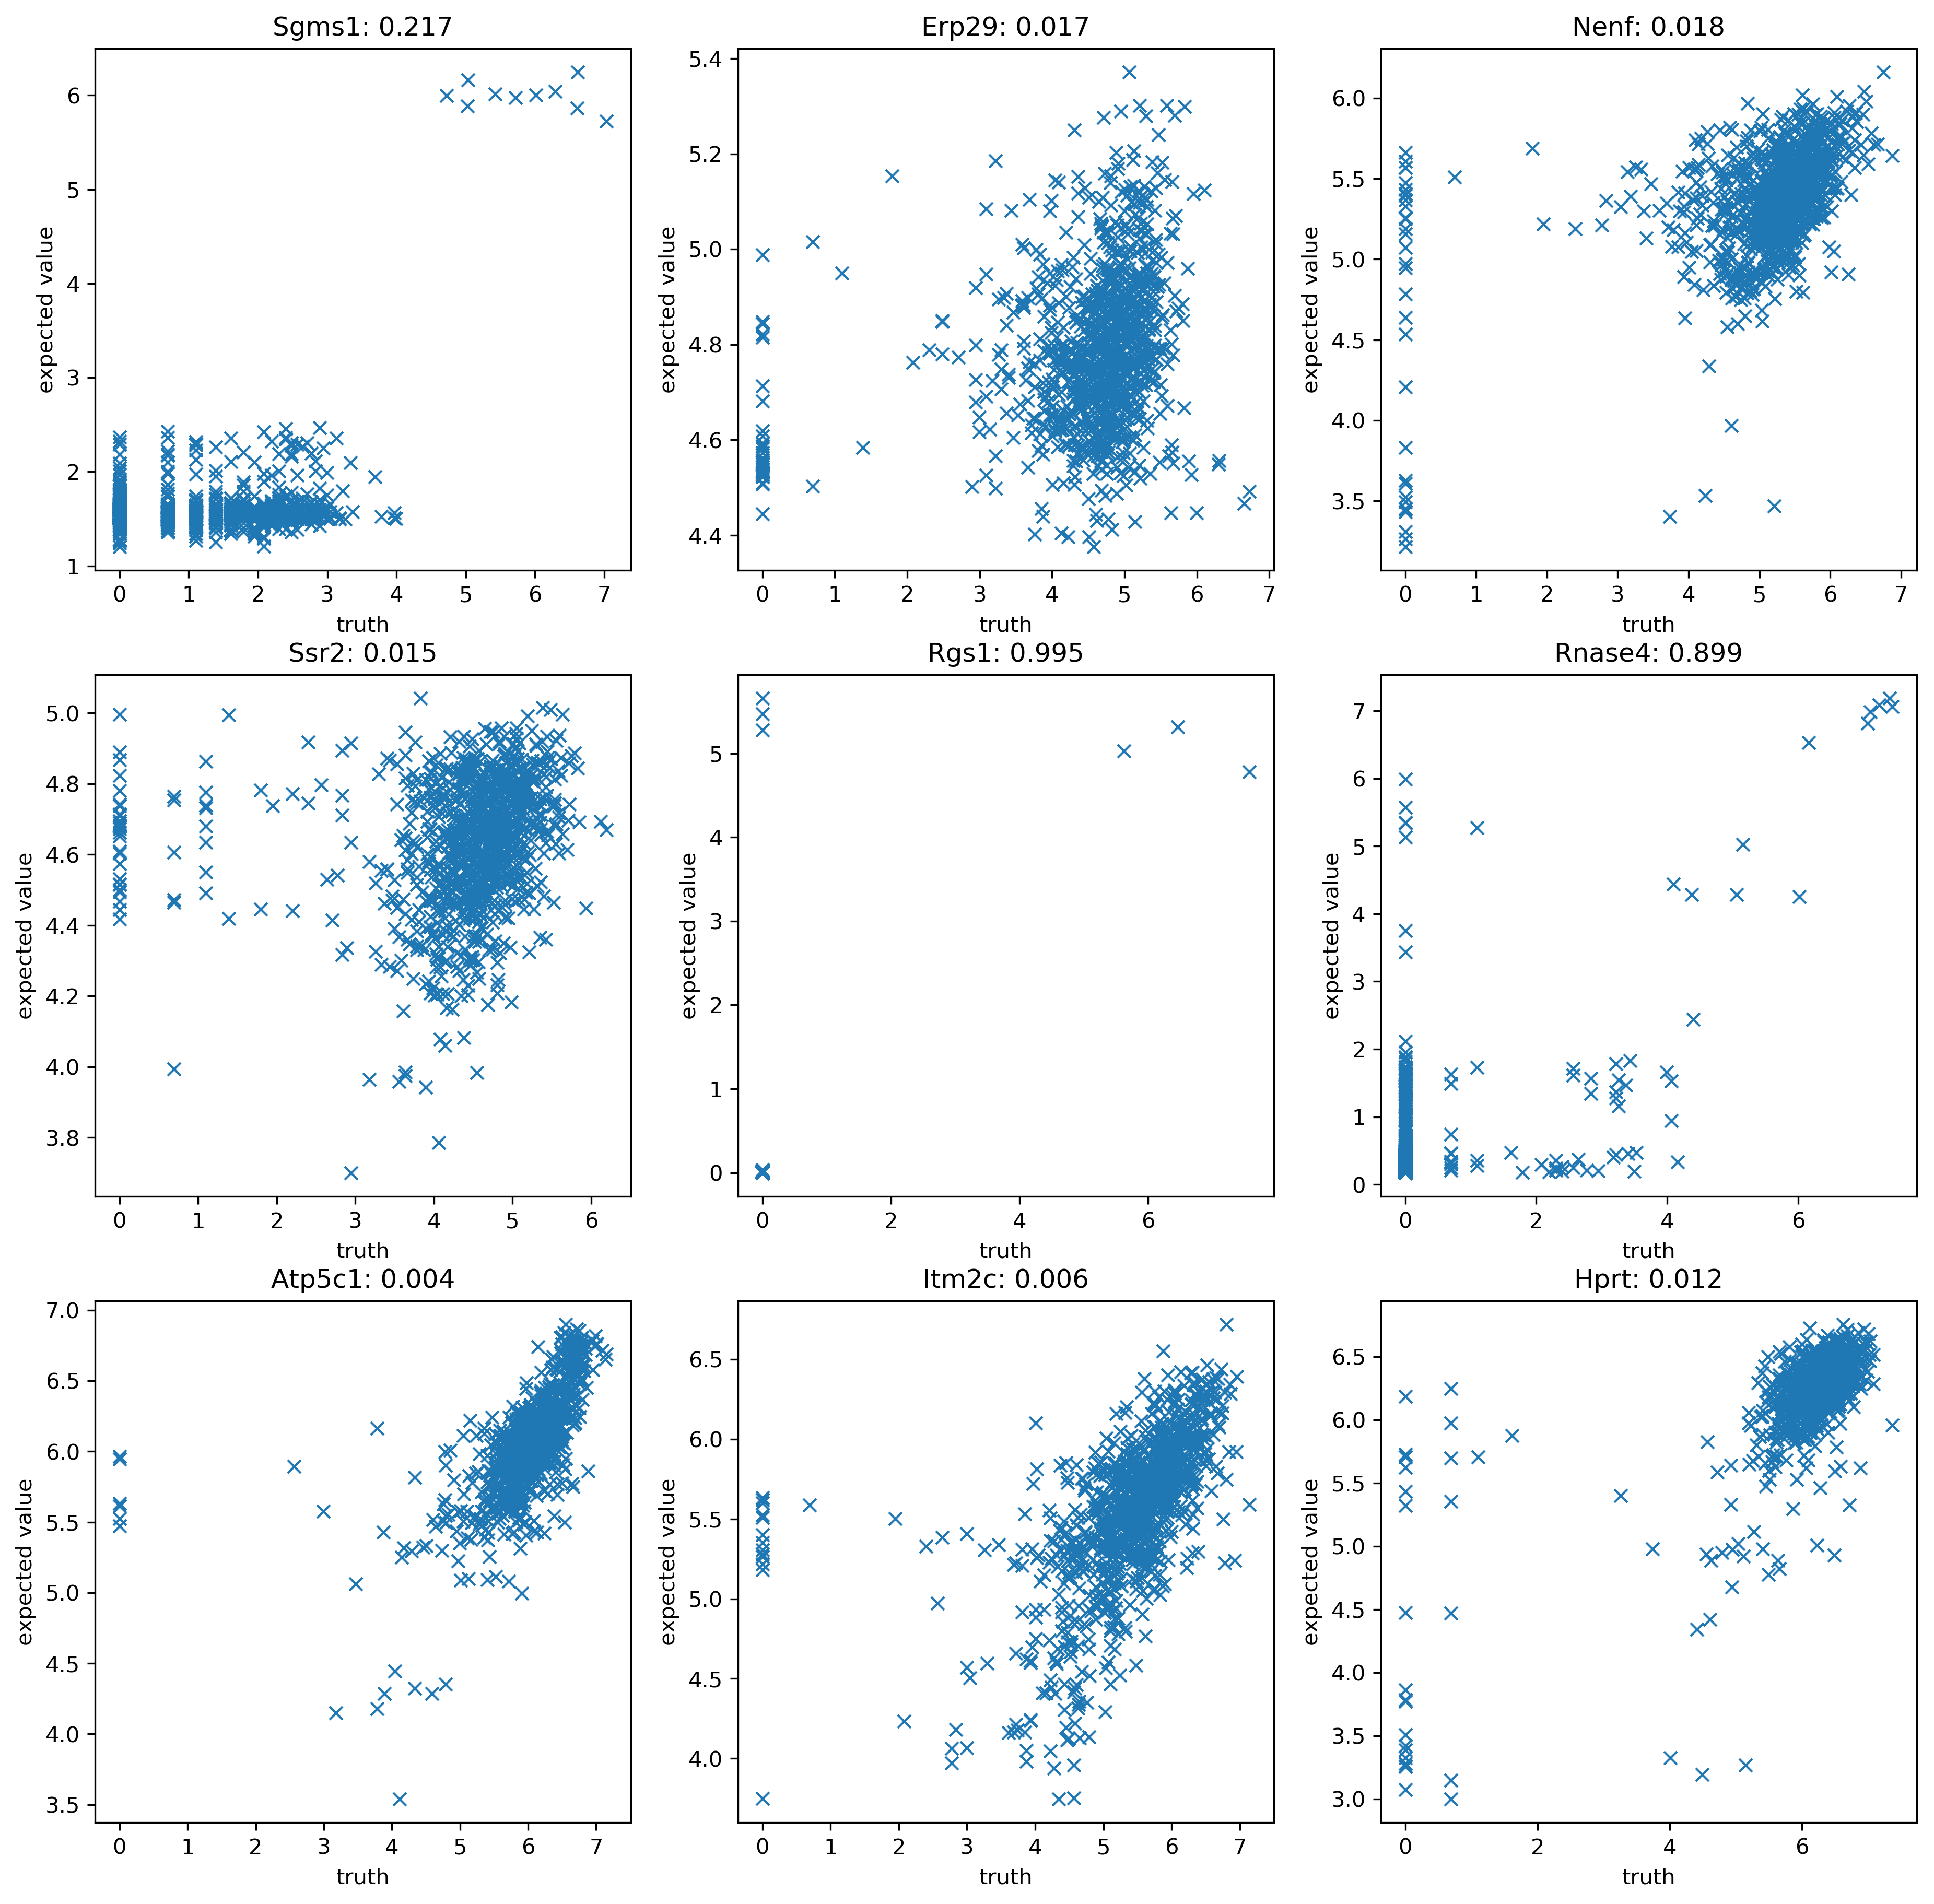
\includegraphics[width=0.8\textwidth]{pics/residsdetail}

One potential reason for this systematic error might be that the negative binomial data distribution is inappropriate.  To diagnose this, we fitted a zero-inflated negative binomial distribution to each collection of cells Allen Institute dubbed a ``cluster.''  We then measured the goodness-of-fit, in terms of whether various moments matched.  In particular, we compared the empirical mean, standard deviation, and proportion of zeros to the corresponding statistics which would be predicted by the learned models.  

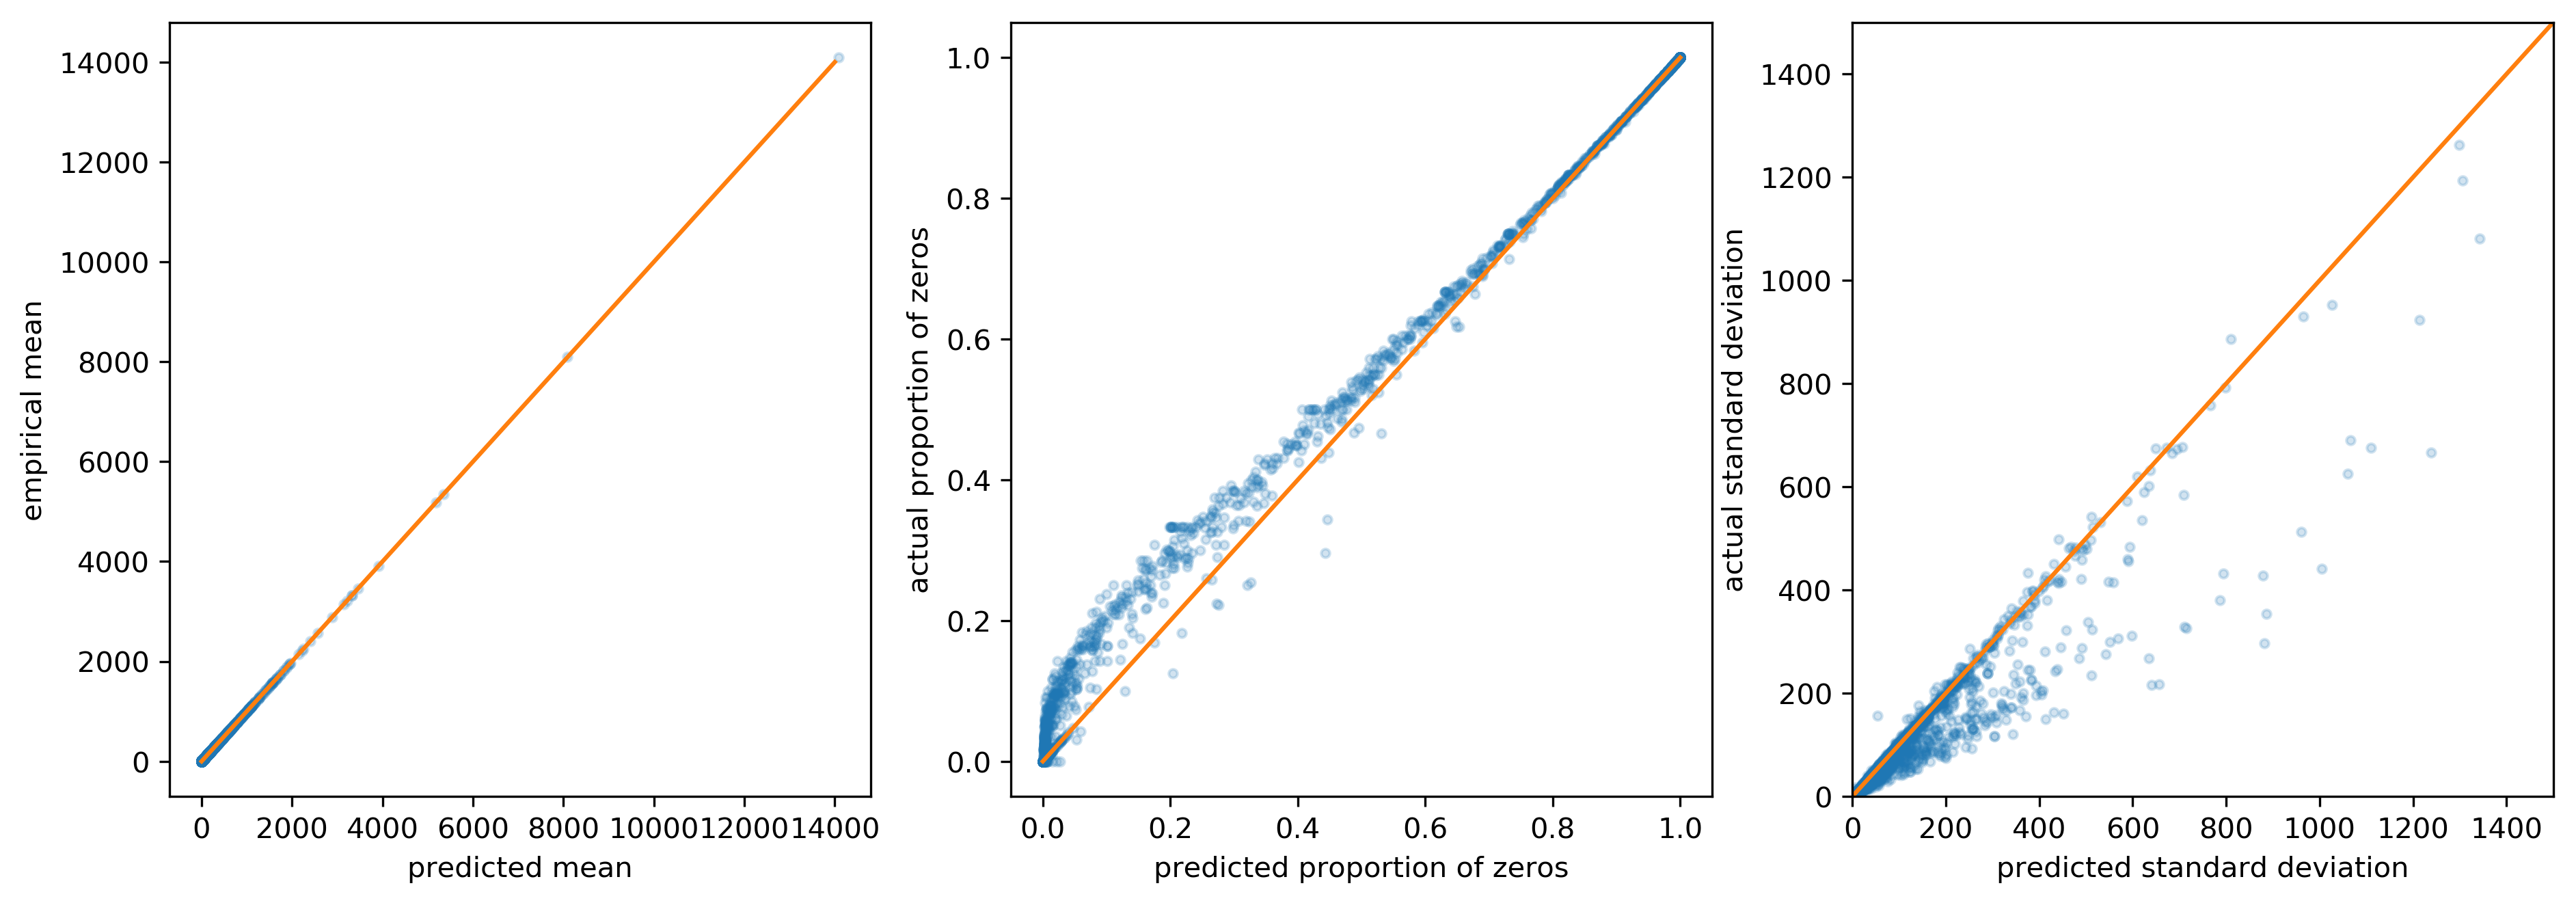
\includegraphics[width=0.8\textwidth]{pics/zinbfitmatch}

In terms of mean and zero proportion, these seem nearly okay, but in terms of variance we can see that we are not doing the greatest job.  For a great many cell types we are predicting standard deviations which are much higher than the reality.  This is perhaps not surprising, since the negative binomial model is inherently overdispersed, and simply cannot accomodate underdispersed data.  

Another possible source of trouble is that in the particular model we use we have made certain assumption about how $\alpha,\beta,h$ can vary.  This could be a big problem.  To see why, we looked at each the fitted parameters of the zero-inflated negative binomial distribution for each cell-type.  This yields a kind of three-dimensional scatterplot, in which each dot is a cell type, and the location indicates the value of each of its three fitted parameters.  Here we show three projections of that scatterplot:

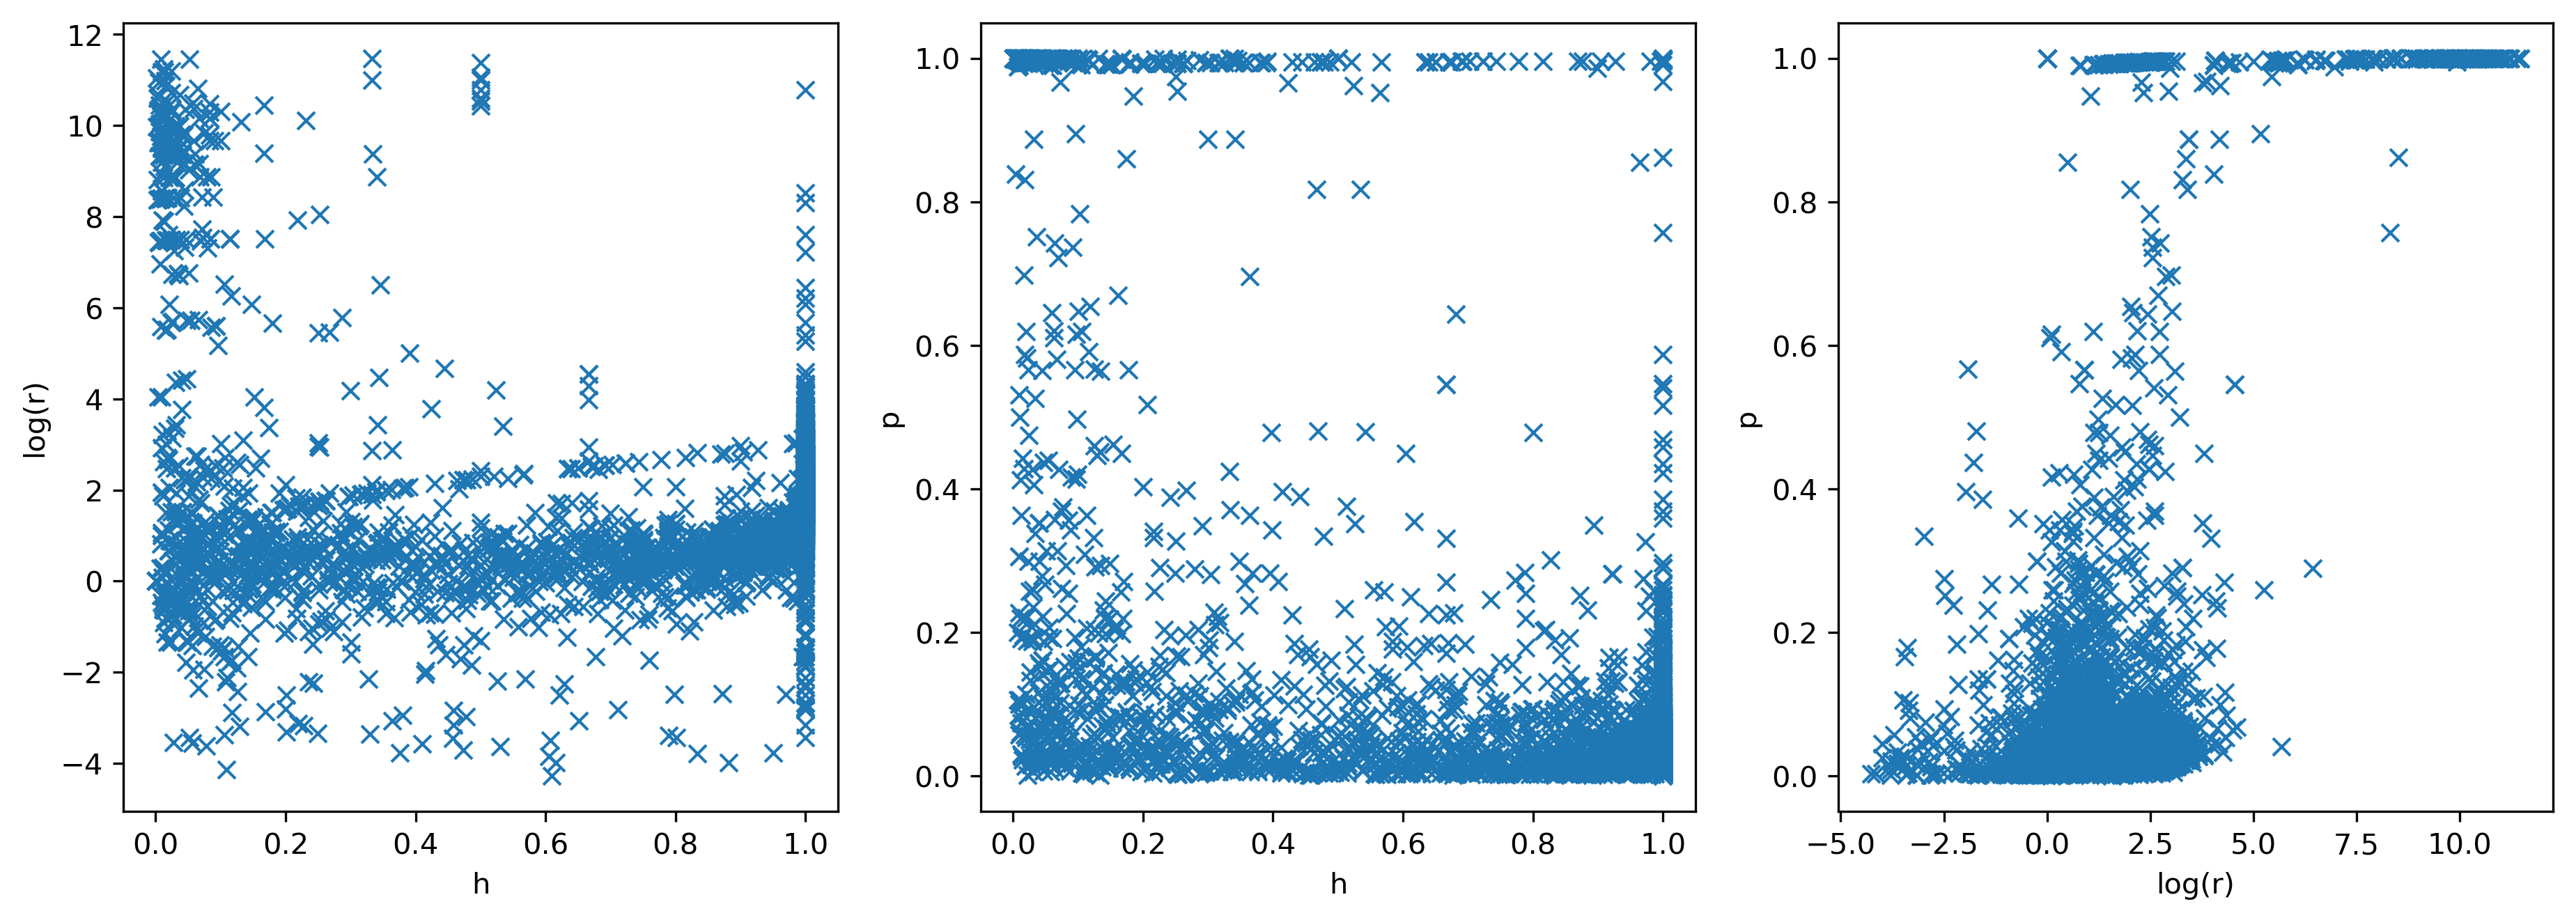
\includegraphics[width=0.8\textwidth]{pics/zinbfitdiversity}

Clearly there is quite a lot of variety in terms of how these parameters may vary.  They do not appear to lie on any kind of low-dimensional manifold.  So we must be very careful in terms of what assumptions our model makes about how these parameters may be tied together.  

% \bibliographystyle{unsrt}
% \bibliography{refs}

\end{document}






































